\documentclass[a4paper]{article}
\usepackage[a4paper, left=25mm, right=25mm, top=25mm, bottom=25mm]{geometry}
%\geometry{paperwidth=210mm, paperheight=2000pt, left=5pt, top=5pt}
\usepackage[utf8]{inputenc}
\usepackage[english,russian]{babel}
\usepackage{indentfirst}
\usepackage{tikz}
\usepackage{cancel}
\usetikzlibrary{automata,positioning,arrows}
\usepackage{amsmath}
\usepackage{enumerate}
\usepackage{hyperref}
\usepackage{amsfonts}
\usepackage{amssymb}
\usepackage{amsthm}
\DeclareMathOperator*{\argmin}{arg\,min}
\DeclareMathOperator*{\argmax}{arg\,max}
\usepackage{wasysym}
\title{Statistical Learning Theory\\Проект (реферат по статье)}
\date{}
\author{Сергей~Володин, 374 гр.}
\newcommand{\matrixl}{\left|\left|}
\newcommand{\matrixr}{\right|\right|}

\newcommand{\sign}{\mbox{sign}\,}
\newcommand{\F}{\mathcal{F}}
\newcommand{\Hh}{\mathcal{H}}
\newcommand{\R}{\mathbb{R}}
\newcommand{\E}{\mathbb{E}}
\newcommand{\N}{\mathbb{N}}
\newcommand{\Be}{\mbox{Be}}
\newcommand{\Reg}{\mbox{Regret}}
\newcommand{\dkl}{d_{\mbox{\tiny KL}}}
\newcommand{\Ss}{\mathcal{S}}
\newcommand{\ltwo}{\log_2 }
\newcommand{\A}{\mathcal{A}}

% пустое слово
\def\eps{\varepsilon}

% регулярные языки
\def\eqdef{\overset{\mbox{\tiny def}}{=}}
\newcommand{\niton}{\not\owns}

\begin{document}
\maketitle
\section{Обучение с подкреплением}
Обучение с подкреплением~--- область машинного обучения, идея которой основана на поведенческой психологии. Рассматривается {\em агент}, взаимодействующий со {\em средой} путем наблюдения ее {\em состояния}, совершения {\em действий} и получения от среды {\em награды}.

\begin{figure}[h]
\caption{Блок-схема обучения с подкреплением}
\centering 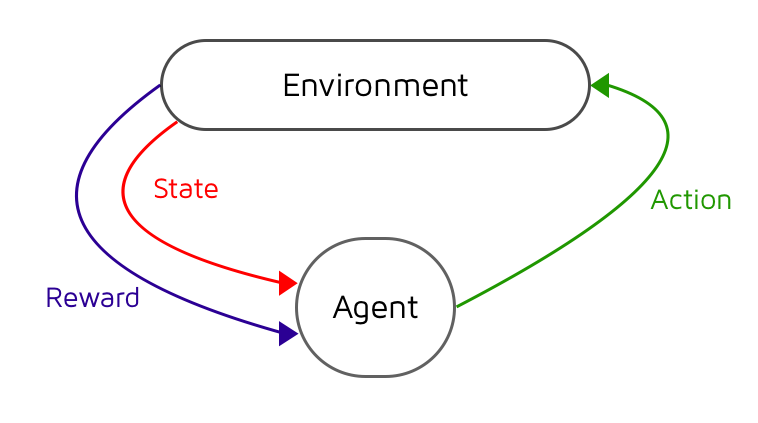
\includegraphics[width=150px]{RL.png}
\label{RL}
\end{figure}

Обучение с подкреплением находится на стыке многих областей, таких как машинное обучение, оптимальное управление и neuroscience.
\begin{figure}[h]
	\caption{Положение обучения с подкреплением. Лекция Дэвида Сильвера \cite{silver}}
	\centering 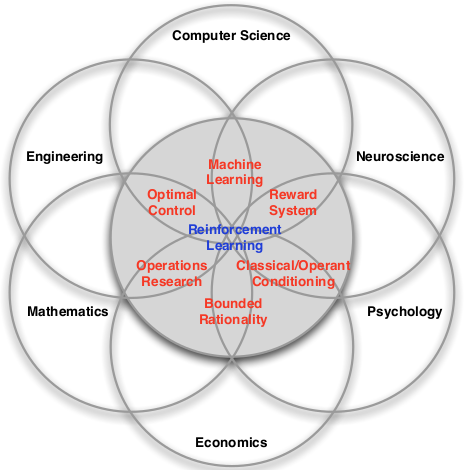
\includegraphics[width=150px]{RL_position_DavidSilver.png}
\end{figure}

В последнее время обучение с подкреплением набирает популярность благодаря успехам в решении важных практические задачи. Например, при помощи обучения с подкреплением удается обучать агентов, способных играть в игры Atari \cite{dqn}, Go \cite{go} и backgammon.

\section{Введение}
Поскольку агент обучается правильным действиям в среде постепенно, сначала он может принимать неоптимальные действия. Таким образом возникает понятие сожаления (regret)~--- величины, характеризующей то, насколько неоптимально агент выбирает действия. Данный реферат рассказывает о статье <<On Lower Bounds for Regret in Reinforcement Learning>> (Ian Osband, Benjamin Van Roy) \cite{lower_bounds}. В статье рассматриваются нижние границы на сожаление. Данная величина характеризует <<сложность>> самой среды в терминах разницы между наградой данного алгоритма и некоего <<наилучшего>> алгоритма обучения с подкреплением.

Далее будут даны необходимые определения, а затем будет рассмотрен пример самой простой среды~--- многорукий бандит. Для нее будет получена нижняя оценка на сожаление.

В оригинальной статье разбирается также случай среды с двумя состояниями, но в данном реферате данный раздел не представлен.

\section{Постановка задачи}

\theoremstyle{definition}
\newtheorem{definition}{Определение}[section]
\newtheorem{lemma}{Лемма}[section]
\newtheorem{theorem}{Теорема}[section]
\begin{definition}{(Марковский процесс принятия решений)}
	
ММПР~--- это кортеж $(\mathcal{S}, \mathcal{A}, R, P)$, где
\begin{enumerate}
	\item $\mathcal{S}=\{1,...,S\}$~--- множество состояний среды
	\item $\mathcal{A}=\{1,...,A\}$~--- множество действий, доступных агенту
	\item $R(s,a)$~--- функция награды. Для данных $s\in \Ss$ и $a\in\A$ случайная величина $R(s, a)\in[0,1]$~--- награда за действие
	\item $P(s,a)$~--- функция переходов. Для данных $s\in \Ss$ и $a\in\A$ случайная величина $P(s, a)\in\Ss$~--- новое состояние среды
\end{enumerate}
\end{definition}

\begin{definition}{(Взаимодействие агента со средой)}

Имеется ММПР $(\Ss,\A,R,P)$. Вводится время $t\in\N$. Для каждого момента времени \ref{RL}:
\begin{enumerate}
\item Агент получает состояние $s_t\in \Ss$
\item Агент выбирает действие $a_t\in\A$
\item Агент получает награду $r_t\sim R(s_t,a_t)\in[0,1]$
\item Среда переходит в новое состояние $s_{t+1}\sim P(s_t,a_t)$
\end{enumerate}
\end{definition}

\begin{definition}{(Политика)}
Имеется ММПР $(\Ss,\A,R,P)$.

Политика $\mu$~--- отображение $\mu\colon \Ss\to\A$. То есть, каждому состоянию $s\in\Ss$ сопоставляется действие агента $a\in\A$
\end{definition}

\begin{definition}{(Средняя награда)}
Имеется ММПР $M=(\Ss, \A,R,P)$, а также политика $\mu$.

$$\lambda_{\mu}^M(s)=\lim\limits_{T\to\infty}\E_{M,\mu}\left[\frac{1}{T}\sum\limits_{t=1}^T\overline{r}(s_t,a_t)\big|s_1=s\right]$$

где $\overline{r}(s,a)=\E R(s,a)$~--- средняя награда в $(s,a)$

То есть, $\lambda_{\mu}^M(s)$~--- средняя награда за бесконечное время при следовании политике $\mu$ в ММПР $M$, если стартовать из состояния $s\in\Ss$. В некотором смысле это <<ценность>> состояния $s$.

Политика $\mu^M$ оптимальна для $M$, если $\mu^M\in\argmax\limits_{\mu}\lambda^M_{\mu}(s)$ для всех $s\in\Ss$. То есть, при старте из любого состояния $s$ политика $\mu$ максимизирует среднюю награду за бесконечное время.

Величина $\lambda_*^M(s)=\lambda_{\mu^M}^M(s)$ называется оптимальной средней наградой.
\end{definition}

\begin{definition}{(История)}
Имеется ММПР $M=(\Ss,\A,R,P)$. История к моменту времени $t$~--- кортеж $$\Hh_t=(s_1,a_1,r_1,...,s_{t-1},a_{t-1},r_{t-1})$$
То есть, это последовательный <<журнал>> всех состояний, действий и наград, которые произошли во время взаимодействия агента со средой.
\end{definition}

\begin{definition}{(Алгоритм обучения с подкреплением)}
Имеется ММПР $M=(\Ss, \A,R,P)$. Алгоритм обучения с подкреплением $\pi$~--- это последовательность функций $\pi=\{\pi_t\big|t\in\N\}$, где $\pi_t$~--- функция, сопоставляющая истории $\Hh_t$ распределение над политиками $\pi_t(\Hh_t)$
	
То есть, алгоритм $\pi$ получает историю $\Hh_t$ в момент времени $t$ и возвращает распределение над политиками $\pi_t(\Hh_t)$. Далее выполняется сэмплинг $\mu_t\sim\pi_t(\Hh_t)$ из этого распределения, и агент возвращает действие $\mu_t(s_t)$.
\end{definition}

\begin{definition}{(Сожаление)}
Имеется ММПР $M=(\Ss, \A,R,P)$ и агент $\pi$.
	
Сожаление агента $\pi$ в момент времени $T$ для начального состояния $s$ в цепи $M$ определяется следующим образом:
$$\Reg(T,\pi,M,s)=\sum\limits_{t=1}^T(\lambda^M_{\mu^M}(s)-r_t)=T\lambda_*^M(s)-\sum\limits_{t=1}^Tr_t$$

То есть, агент взаимодействует со средой, которая изначально находится в состоянии $s$ в течение $T$ шагов времени. В этом процессе им получаются награды $\{r_i\}_{i=1}^T$.

За всё время $T$ агент мог бы действовать оптимально. Тогда можно ожидать, что он бы получил около $T\lambda_*^M(s)$ награды, так как $\lambda_*^M$~--- средняя награда для состояния $s$. Вместо этого он получил только $\sum\limits_{t=1}^Tr_t$.

Заметим, что $\Reg(T,\pi,M,s)$~--- случайная величина (случайность берётся как из недетерминированности агента, так и из недетерминированности среды)
\end{definition}

\section{Многорукие бандиты}
\begin{definition}{(Многорукий бандит)}
Многорукий бандит $M$~--- ММПР с всего одним состоянием: $S=1$. Действия $a\in\A$ называются <<руками>>.

Для многорукого бандита оптимальная средняя награда вырождается в максимальное $\overline{r}(a)$:
$$\lambda_*^M=\max\limits_a\overline{r}(a)$$

То есть, один раз выбирается действие, для которого средняя награда $\overline{r}$ максимальна и повторяется каждый раз.
\end{definition}

\begin{theorem}{(Нижняя граница на сожаление для многоруких бандитов)}

Имеется многорукий бандит $M$. Тогда для любого алгоритма обучения с подкреплением $\pi$ существует функция награды $R$, такая что
$$\E\Reg(T,\pi,M)\geqslant \frac{1}{24}\sqrt{AT}$$
\end{theorem}

Доказательству этой теоремы посвящен остаток этого раздела.

Рассмотрим следующую среду: пусть $M$~--- многорукий бандит с $A\geqslant 2$ и следующей функцией награды:
$$
R(a)=\begin{cases}
\Be(\delta),&a\neq a^*\\
\Be(\delta+\eps),&a=a^*
\end{cases}
$$

То есть, все <<руки>> одинаковые и имеют распределение награды по Бернулли с параметром $\delta$, кроме руки $a^*$, имеющей распределение $\Be(\delta+\eps)$.

Определяется изменённая награда
$$\tilde{r}_t(a)=\begin{cases}
r_t(a),&a\neq a^*\\
\sim \Be(\delta),&a=a^*
\end{cases}$$

То есть, награда для действий, отличных от $a^*$ остается без изменений. Для действия $a^*$ производится дополнительный сэмплинг из независимого распределения $\Be(\delta)$. Заметим, что распределение такой награды $\tilde{r}_t(a)$ всегда является $\Be(\delta)$. То есть, она никак не информирует агента о преимуществе $a^*$ перед другими действиями.

Рассматривается изменённая история для $\tilde{a}_t\sim\pi_t(\tilde{\Hh}_t)$
$$\tilde{\Hh}_t=(\tilde{a}_1,\tilde{r}_1,...,\tilde{a}_{t-1},\tilde{r}_{t-1})$$

В этой истории агент получает измененную награду $\tilde{r}_t$, которая никак не информирует его о том, что рука $a^*$ <<лучше>>, чем остальные.

Определяются величины $n_T(a)=\sum\limits_{t=1}^T[a_t=a]$ и $\tilde{n}_T(a)=\sum\limits_{t=1}^T[\tilde{a}_t=a]$~--- количества выборов действия $a$ в историях $\Hh_{T+1}$ и $\tilde{\Hh}_{T+1}$ соответственно.
\begin{lemma}{(Сожаление неинформированного агента)}

Рассмотрим построенного многорукого бандита $M$. Для всех $\delta,\,\eps>0$ и всех алгоритмов обучения с подкреплением $\pi$ сожаление
$$R_u=T\lambda_*^M(a)-\E\sum\limits_{t=1}^Tr(\tilde{a}_t)\geqslant\frac{A-1}{A}T\eps$$
\end{lemma}

\begin{proof}
	
Рассмотрим $T\lambda_*^M=T\max\limits_a\overline{r}(a)$. Тогда $$R_u=\E_{\mbox{agent}}\sum\limits_{t=1}^T \E_{\mbox{env}}[r(a^*)-r(\tilde{a}_t)]$$

Эта разница равна $\eps$ каждый раз, когда $\tilde{a}_t\neq a^*$ и $0$ в противном случае. Перепишем сумму как сумму по действиям и количеству действий:

$$R_u=\E\sum\limits_{a} \tilde{n}_T(a)(\overline{r}(a^*)-\overline{r}(a))=\E\sum\limits_{a\neq a^*}\eps \tilde{n}_T(a)=\E \eps(T-\tilde{n}_T(a^*))=\eps T\frac{A-1}{A}$$

Где последний шаг произведен из соображений симметрии:

$$\E \tilde{n}_T(a^*)=\frac{T}{A}$$

Симметрия возникает, поскольку агент не может отличить $a^*$ от других действий, получая награду $\tilde{r}_t$.
\end{proof}

Перейдём к следующему этапу доказательства Теоремы 1. В этой части докажем следующее утверждение: если $\eps$ достаточно мал, тогда распределение награды $\tilde{r}_t(a_t)$ близко к $r_t(a_t)$.

\begin{definition}{(Total variation distance)}

Пусть $(\Omega,\mathcal{F},P)$ и $(\Omega,\mathcal{F},Q)$~--- два вероятностных пространства.

Тогда total variation distance между $P$ и $Q$ определяется как:

$$\delta(P,Q)=\sup\limits_{A\in\mathcal{F}}|P(A)-Q(A)|$$
	
То есть, это максимальный модуль разности мер по всем измеримым подмножествам.

Аналогично total variation distance определяется для случайных величин
\end{definition}

\begin{definition}{(Расхождение Кульбака-Лейблера)}
Пусть $P$ и $Q$~--- два распределения. Тогда расхождением Кульбака-Лейблера $Q$ относительно $P$ называется
$$\dkl(P||Q)=\int\limits_Xp(x)\ltwo\frac{p(x)}{q(x)}dx$$
\end{definition}

\begin{theorem}{(Неравенство Пинскера)}
Пусть $P$, $Q$~--- две случайные величины.

Тогда
$$\delta(P,Q)\leqslant\sqrt{\frac{1}{2}\dkl(P||Q)}$$
\end{theorem}

\begin{proof}
См. \cite{pinsker}
\end{proof}

Определим две последовательности наград:
$$\begin{cases}
r_t^T=(r_t,...,r_T)\\
\tilde{r}_t^T=(\tilde{r}_t,...,\tilde{r}_T)
\end{cases}$$

Определим условное распределение последовательностей наград $r_t^T$ и $\tilde{r}_t^T$ при заданной истории в точке $z_t^T\in\R^{T-t+1}$
$$
\begin{cases}
P(z_t^T|\Hh_t)=\mathbb{P}(r_t^T=z_t^T\big| \Hh_t)\\
\tilde{P}(z_t^T\big|\tilde{\Hh}_t)=\mathbb{P}(\tilde{r}_t^T=z_t^T\big|\tilde{\Hh}_t)
\end{cases}
$$

Рассмотрим матожидание расхождения Кульбака-Лейблера $P(z_t^T|\Hh_t)$ относительно $\tilde{P}(z_t^T|\tilde{\Hh}_t)$:

$$d_t^T=\dkl(\tilde{P}(z_t^T|\tilde{\Hh}_t)||P(z_t^T|\Hh_t)=\E\sum\limits_{z_t^T}\tilde{P}(z_t^T|\tilde{\Hh}_t)\ltwo\frac{\tilde{P}(z_t^T|\tilde{\Hh}_t)}{P(z_t^T|\Hh_t)}$$

\begin{lemma}{(КЛ-расхождение неинформированного распределения)}

Рассмотрим построенного многорукого бандита $M$. Для всех $\eps,\,\delta>0$ и всех алгоритмов обучения с подкреплением $\pi$

$$d_1^T\leqslant \frac{T}{A}\left(\delta\ltwo\frac{\delta}{\delta+\eps}+(1-\delta)\ltwo\frac{1-\delta}{1-\delta-\eps}\right)$$
\end{lemma}

\begin{proof} По цепному правилу для расхождения Кульбака-Лейблера \cite{bubeck}, \cite{games}
$$d_t^T=\sum\limits_{t=1}^T d_t^t$$

Поскольку награда $\tilde{r}_t$ всегда распределена по $\Be(\delta)$, $$\tilde{P}(z_t^t)=\begin{cases}
\delta, & z_t^t=1\\
1-\delta, & z_t^t=0
\end{cases}$$

Для $r_t$ распределение зависит от действия. Для $a\neq a^*$ распределение совпадает с $\tilde{P}$. Но для $a=a^*$
$$P(z_t^t)=\begin{cases}
\delta+\eps, & z_t^t=1\\
1-\delta-\eps, & z_t^t=0
\end{cases}$$

Эти числа как раз стоят в верхней оценке. Дополнительные вычисления \cite{bubeck} дают:

$$d_1^T\leqslant\sum\limits_{t=1}^T P(\tilde{a}_t= a^*)\left(\delta\ltwo\frac{\delta}{\delta+\eps}+(1-\delta)\ltwo\frac{1-\delta}{1-\delta-\eps}\right)$$

Поскольку действия $\tilde{a}_t$ выбираются без информации о различии между <<руками>>, используем тот же прием, использующий симметрию: $$P(\tilde{a}_t\neq a^*)=\frac{A-1}{A}$$
\end{proof}

Теперь мы покажем, что если распределение $P$ близко к $\tilde{P}$, то получающееся сожаление близко к сожалению неинформированного агента:

\begin{lemma}{(Ограничение на сожаление в терминах КЛ-расхождения)}
Пусть $M$~--- построенный многорукий бандит. Тогда для любого $\eps,\,\delta>0$ и для любого алгоритма обучения с подкреплением $\pi$
$$
R=T\max\limits_a\overline{r}(a)-\E\sum\limits_{t=1}^T\overline{r}(a_t)\geqslant \eps T \left(1-\frac{1}{A}-\sqrt{\frac{1}{2}\dkl(\tilde{P}(z_1^T)||P(z_1^T))}\right)
$$
\end{lemma}

\begin{proof}
По неравенству Пинскера \cite{bubeck}:
$$
\E\left[\frac{n_T(a^*)}{T}-\frac{\tilde{n}_T(a^*)}{T}\right]\leqslant\sqrt{\frac{1}{2}\dkl(\tilde{P}(z_1^T||P(z_1^T))}
$$

Далее, поскольку $\E \tilde{n}_T(a^*)=\frac{T}{A}$ из симметрии, получаем

$$\E\frac{n_t(a^*)}{T}\leqslant\sqrt{\frac{1}{2}\dkl(\tilde{P}||P)}+\frac{1}{A}$$

Далее рассуждения аналогичны рассуждениям в доказательстве Леммы 4.1:
$$R=\E\sum\limits_{a\neq a^*}n_T(a)\eps=\eps(T-n_T(a^*))\geqslant \eps T\left(1-\frac{1}{A}-\sqrt{\frac{1}{2}\dkl(\tilde{P}||P)}\right)$$
\end{proof}

Далее, оценим величину в Лемме 4.2.

\begin{lemma}{(Ограничение на КЛ-расхождение)}

Рассмотрим функцию $$f(\delta,\eps)=\delta\ltwo\frac{\delta}{\delta+\eps}+(1-\delta)\ltwo\frac{1-\delta}{1-\delta-\eps}$$

При $\delta\in[0,\frac{1}{2}]$ и $\eps\leqslant 1-2\delta$ значение $f(\delta,\eps)\leqslant\frac{\eps^2}{\delta\ln 2}$.
\end{lemma}

\begin{proof}
См. \cite{jaksch} (используется первая производная)
\end{proof}

Теперь докажем Теорему 1.

\begin{proof}{(Теорема 1)}
Рассмотрим
$$R=T\max\limits_a \overline{r}(a)-\E\sum\limits_{t=1}^T\overline{r}(a_t)$$

По Лемме 4.3

$$
R\geqslant\eps T \left(1-\frac{1}{A}-\sqrt{\frac{1}{2}\dkl(\tilde{P}(z_1^T)||P(z_1^T))}\right)
$$

По Лемме 4.2
$$
\dkl(\tilde{P}||P)\leqslant\frac{T}{A}\left(\delta\ltwo\frac{\delta}{\delta+\eps}+(1-\delta)\ltwo\frac{1-\delta}{1-\delta-\eps}\right)
$$

Значит, по Лемме 4.4
$$
\dkl(\tilde{P}||P)\leqslant \frac{T}{A}\frac{\eps^2}{\delta\ln 2}
$$

Выбираем $\eps^2=\frac{\delta A}{8T}$, подставляем последнюю оценку в оценку $R$:

$$
R\geqslant \eps T(1-\frac{1}{A}-\frac{1}{\sqrt{16\ln 2}})\geqslant c_0\sqrt{\delta AT}
$$
\end{proof}

\begin{thebibliography}{9}
	\bibitem{lower_bounds} 
	Ian Osband, Benjamin Van Roy
	\textit{On Lower Bounds for Regret in Reinforcement Learning}. 
	arxiv.org: \href{https://arxiv.org/pdf/1608.02732.pdf}{paper in pdf}
	
	\bibitem{silver} 
	David Silver
	\textit{UCL Course on RL}.
	\href{http://www0.cs.ucl.ac.uk/staff/d.silver/web/Teaching.html}{slides}
	
	\bibitem{dqn} 
	Volodymyr Mnih et al.
	\textit{Playing Atari with Deep Reinforcement Learning}.
	\href{https://www.cs.toronto.edu/~vmnih/docs/dqn.pdf}{paper in pdf}

	\bibitem{go} 
	AlphaGo article on
	\href{https://en.wikipedia.org/wiki/AlphaGo}{Wikpedia}

	\bibitem{bubeck} 
	Sebastien Bubeck, Nicolo Cesa-Bianchi
	\textit{Regret analysis of stochastic and nonstochastic multi-armed bandit problems}
	\href{https://arxiv.org/pdf/1204.5721.pdf}{paper in pdf}
	
	\bibitem{games} 
	Nicolo Cese-Bianchi, Gabor Lugosi
	\textit{Prediction, Learning, and Games}
	\href{http://www.ii.uni.wroc.pl/~lukstafi/pmwiki/uploads/AGT/Prediction_Learning_and_Games.pdf}{book in pdf}	

	\bibitem{pinsker} 
	Khudanpur Sanjeev, Yaqiao Li
	\textit{Information theoretic methods in statistics (scribe)}
	\href{http://www.cs.mcgill.ca/~yli252/files/Pinsker.pdf}{pdf}

	\bibitem{jaksch} 
	Thomas Jaksch et al.
	\textit{Near-optimal Regret Bounds for Reinforcement Learning}
	\href{http://www.jmlr.org/papers/volume11/jaksch10a/jaksch10a.pdf}{pdf}	
	
\end{thebibliography}
\end{document}